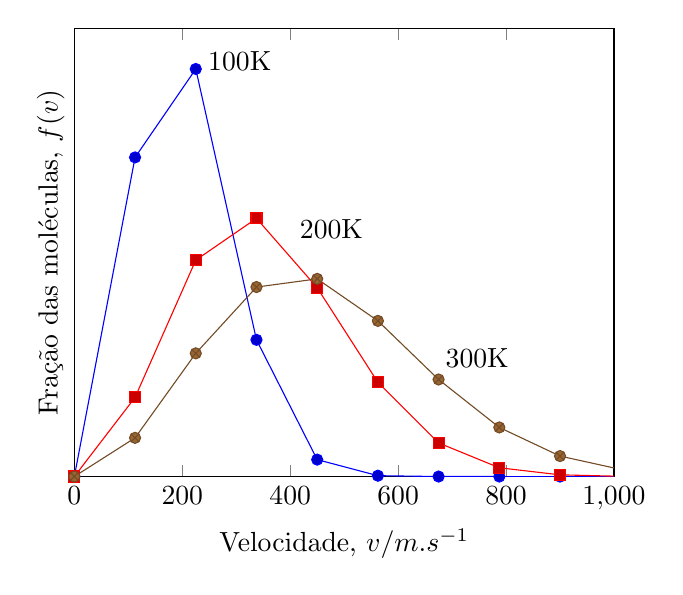
\begin{tikzpicture}
  \def\R{1000*8.314}% boltzmann constant
  \begin{axis}
    [
      grid = none,
      domain = 0:2700,
      xlabel = {Velocidade, $v/\unit{m.s^{-1}}$},
      ylabel = {Fração das moléculas, $f(v)$},
      xmin=0, ymin=0,
      ytick = \empty,
      xmax=1000,
    ]

  \pgfplotsinvokeforeach{ 100, 300, 500 }
    {
      \addplot
        {
            sqrt(2/pi)*(50/(\R*#1))^(3/2)*x^2*exp(-50/(\R*#1)*x^2/2)
        };
    }

  \node [anchor = south west] at (axis cs:230,0.004) 
    { \qty{100}{K} };
  \node [anchor = south west] at (axis cs:400,0.0023) 
    { \qty{200}{K} };
  \node [anchor = south west] at (axis cs:670,0.001) 
    { \qty{300}{K} };
\end{axis}
\end{tikzpicture}